%%%%%%%%%%%%%%%%%%%%%%%%%%%%%%%%%%%%%%
% Graphs
%%%%%%%%%%%%%%%%%%%%%%%%%%%%%%%%%%%%%%
\clearpage
\section{Graphs}

\begin{figure}[ht]
    \caption{Comparing Synthetic Data Generators (pMSE)}
    \label{fig:graph_fidelity_compare}
    \centering

    \begin{subfigure}{\textwidth}
        \caption{pMSE}
        \resizebox{\textwidth}{!}{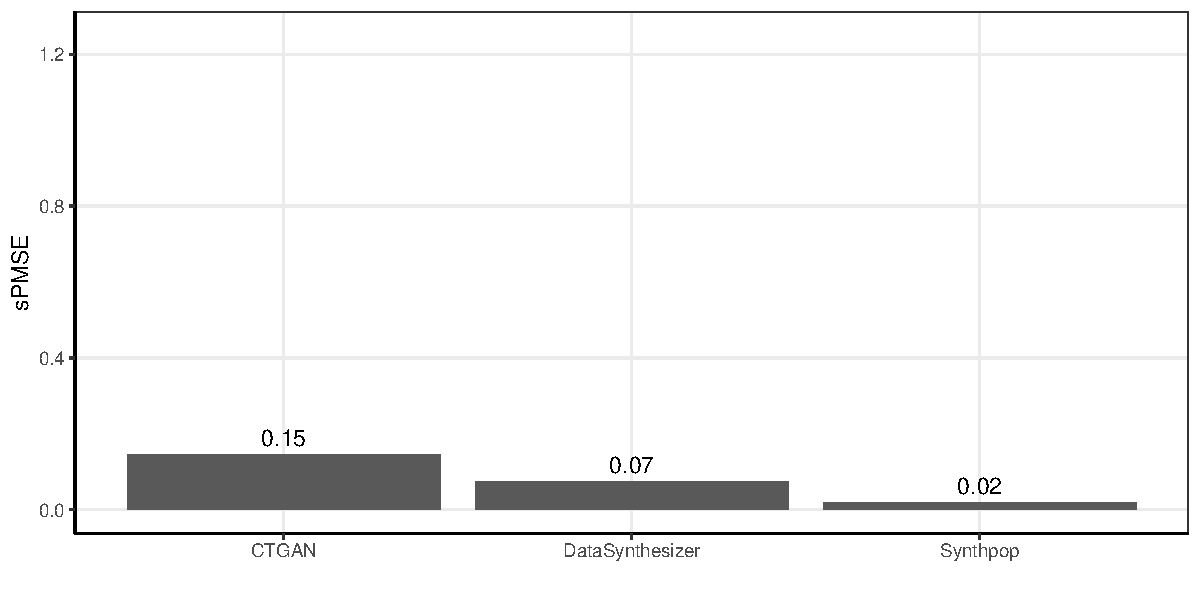
\includegraphics{../graphs/graph_fidelity_compare_dataset.pdf}}
        \label{subfig:graph_fidelity_compare_dataset}
    \end{subfigure}

    \begin{subfigure}{\textwidth}
        \caption{Two-way pMSE}
        \resizebox{\textwidth}{!}{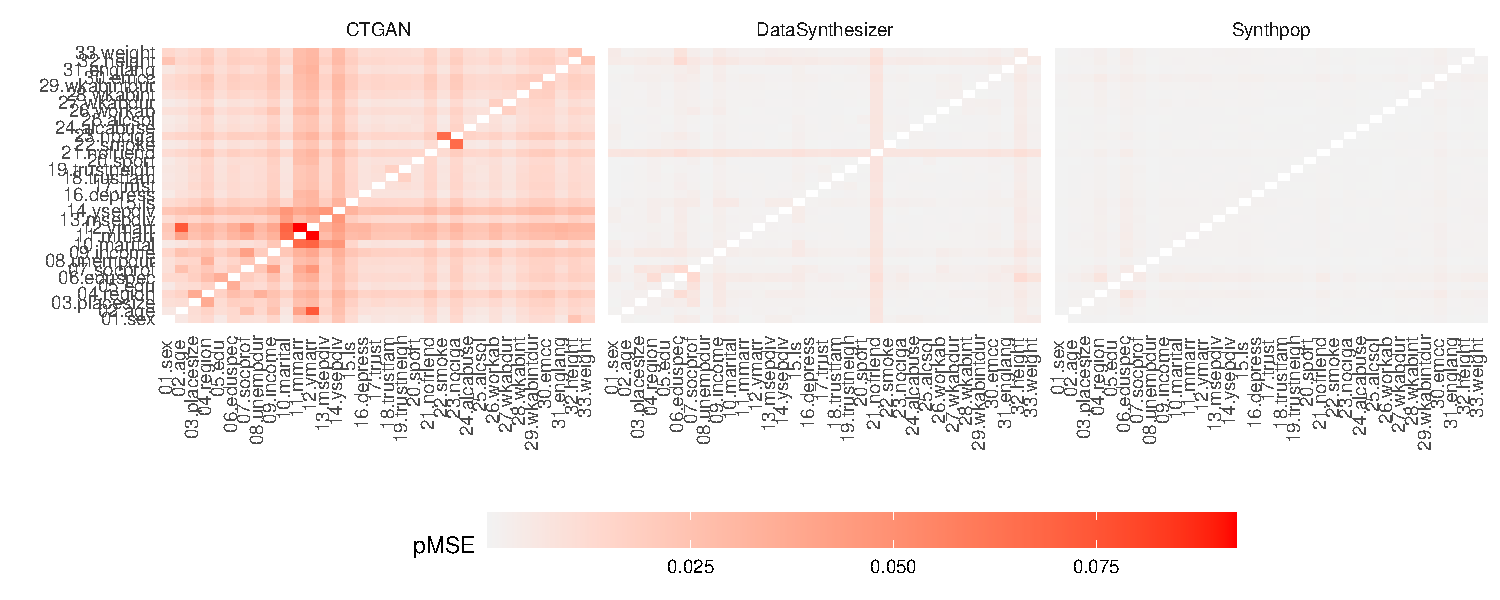
\includegraphics{../graphs/graph_fidelity_twoway_compare.pdf}}
        \label{subfig:graph_fidelity_compare_twoway}
    \end{subfigure}
\end{figure}


\begin{figure}[ht]
    \caption{Comparing one-way frequency of select variables and ROE}
    \label{fig:graph_frequency_compare}
    \centering

    \begin{subfigure}{\textwidth}
        \centering        
        \caption{Number of friends}
        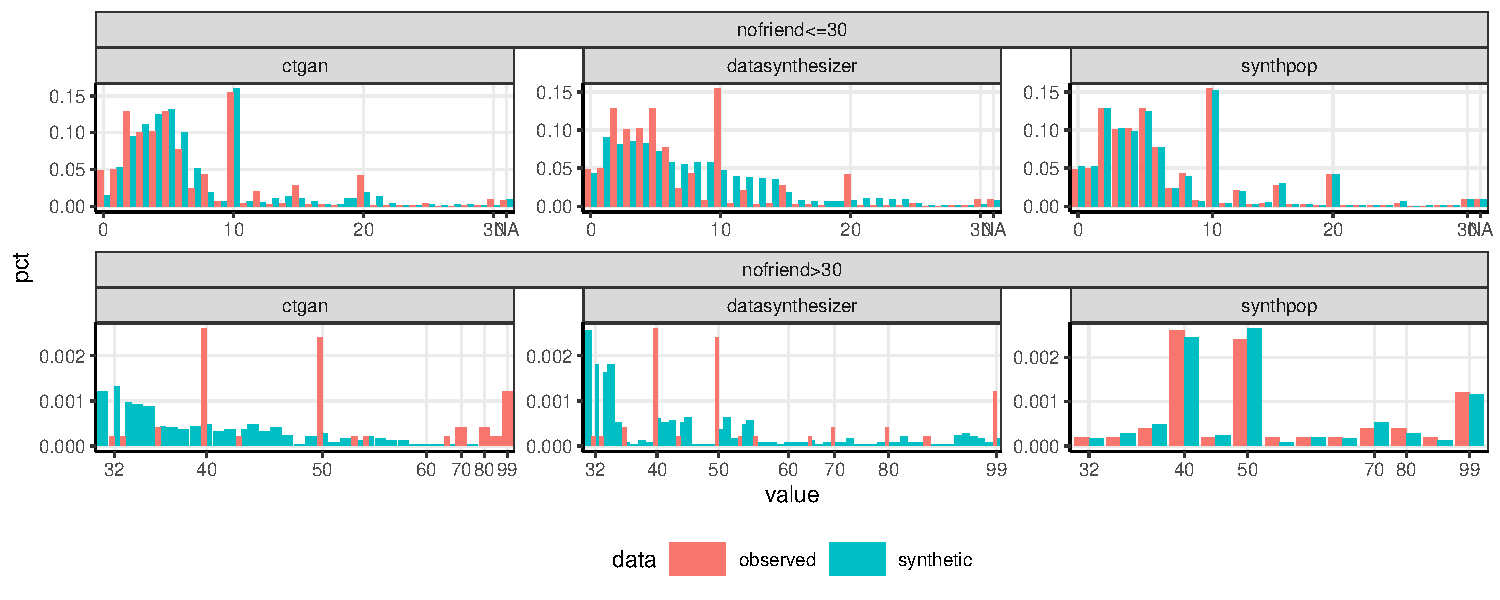
\includegraphics[width=.9\linewidth]{../graphs/compare_nofriend_1.pdf}
        \label{subfig:graph_frequency_compare_nofriend}
    \end{subfigure}

    \begin{subfigure}{\textwidth}
        \centering        
        \caption{BMI}
        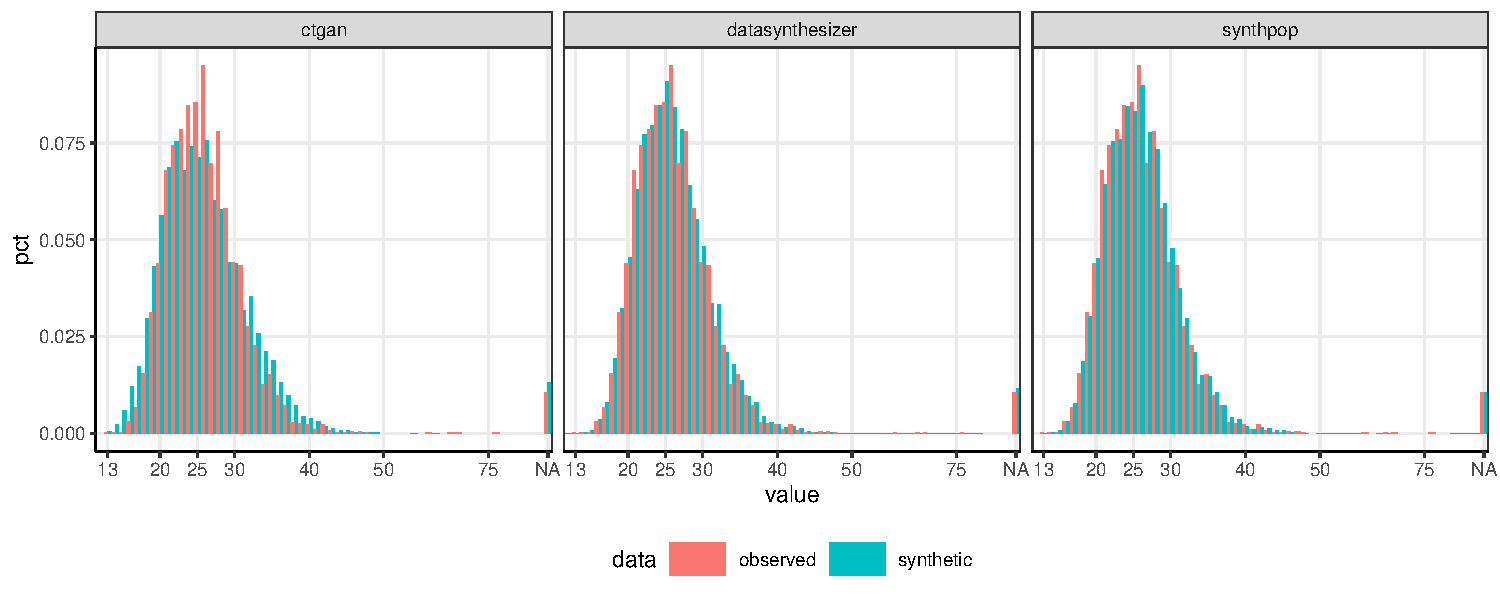
\includegraphics[width=.9\linewidth]{../graphs/compare_bmi_1.pdf}
        \label{subfig:graph_frequency_compare_bmi}
    \end{subfigure}

    \begin{subfigure}{\textwidth}
        \centering        
        \caption{Work abroad duration}
        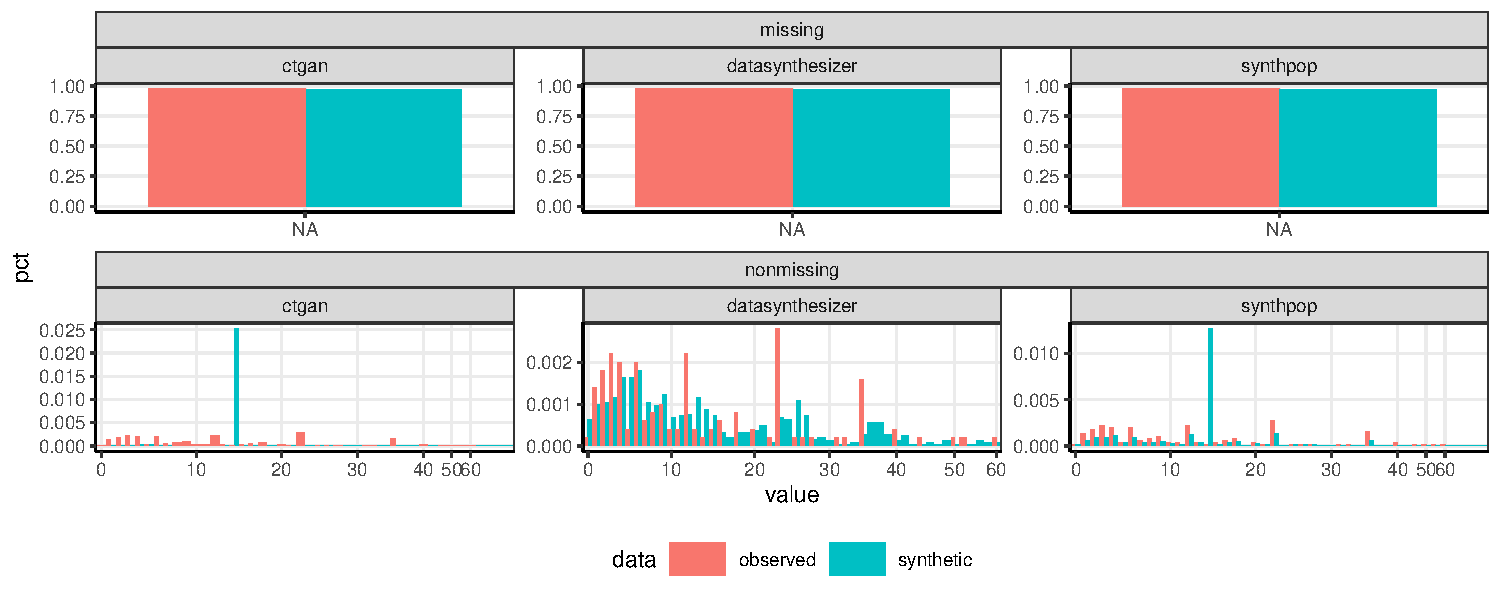
\includegraphics[width=.9\linewidth]{../graphs/compare_wkabdur_1.pdf}
        \label{subfig:graph_frequency_compare_wkabdur}
    \end{subfigure}

    \begin{subfigure}{\textwidth}
        \centering        
        \caption{Education}
        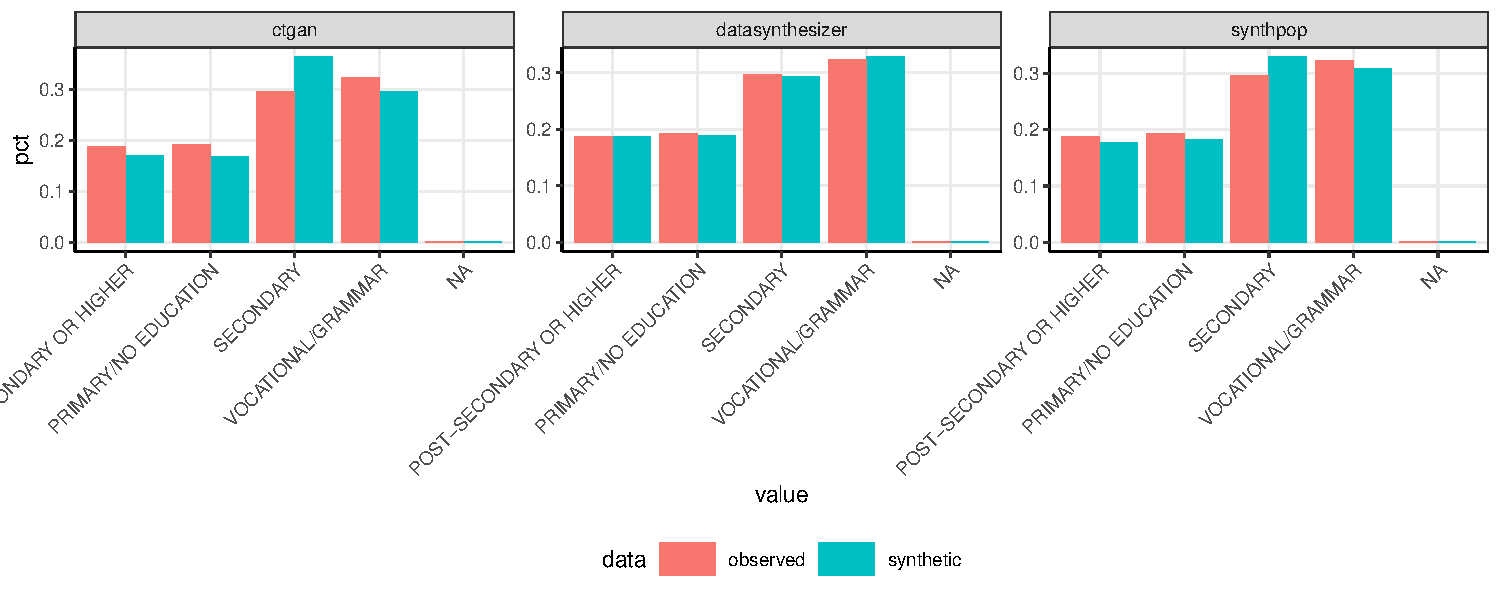
\includegraphics[width=.9\linewidth]{../graphs/graph_frequency_compare_edu.pdf}
        \label{subfig:graph_frequency_compare_edu}
    \end{subfigure}

    % \begin{subfigure}{\textwidth}
    %     \centering        
    %     \caption{Ratio of estimates (ROE)}
    %     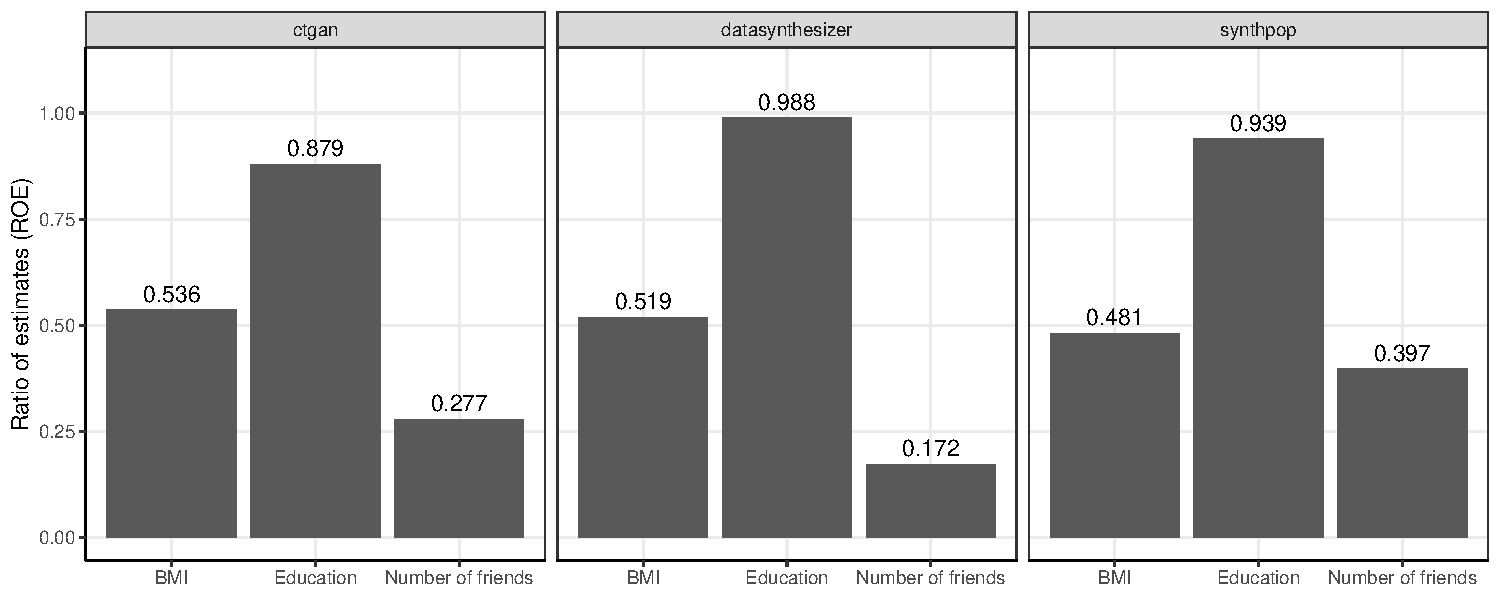
\includegraphics[width=\linewidth]{../graphs/graph_compare_roe.pdf}
    %     \label{subfig:graph_compare_roe}
    % \end{subfigure}
\end{figure}

\begin{figure}
    \caption{Confidence interval overlap}
    \resizebox{\textwidth}{!}{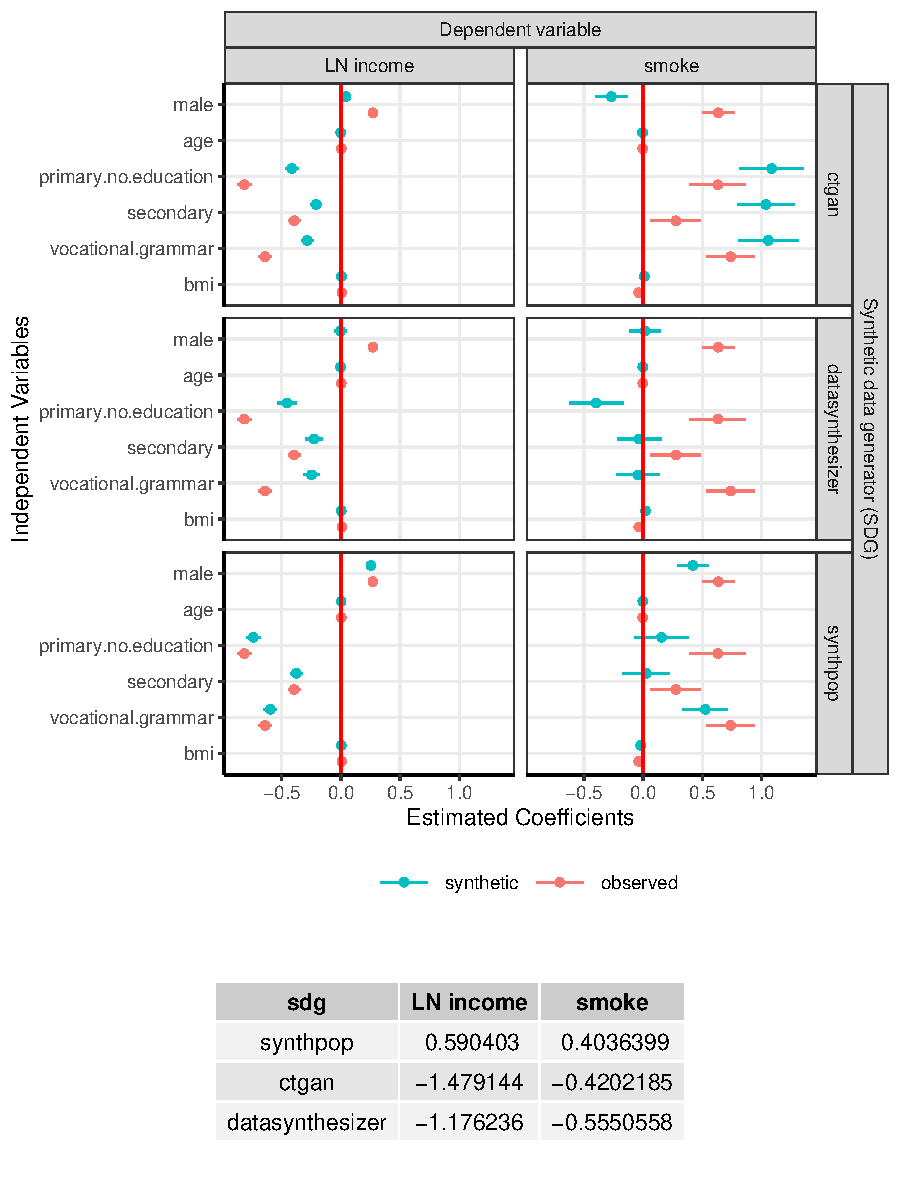
\includegraphics{../graphs/graph_utility_regression_cio_both.pdf}}
    \label{fig:utility_compare_cio}
\end{figure}
